\documentclass[UTF8,fontset=fandol,zihao=-4,a4paper]{ctexart}
\usepackage[margin=21mm,top=23mm,bottom=21mm,headheight=15pt]{geometry}
\usepackage{amsmath,amssymb,graphicx,xcolor,booktabs,array,tabularx,fancyhdr}
\usepackage[unicode,colorlinks=true,linkcolor=blue!48!black,citecolor=blue!48!black,urlcolor=blue!48!black]{hyperref}
\definecolor{Ink}{HTML}{213247}
\definecolor{Accent}{HTML}{176C78}
\definecolor{Pale}{HTML}{EDF5F5}
\definecolor{Muted}{HTML}{4D5C6D}
\renewcommand{\arraystretch}{1.27}
\setlength{\parskip}{3pt}
\setlength{\emergencystretch}{2em}
\ctexset{section={format=\Large\sffamily\bfseries\color{Ink},beforeskip=10pt,afterskip=6pt},
subsection={format=\large\sffamily\bfseries\color{Accent},beforeskip=7pt,afterskip=4pt}}
\pagestyle{fancy}
\fancyhf{}
\fancyhead[L]{\small\color{Muted}Kohn–Sham 方程与原子中心高斯基}
\fancyhead[R]{\small\color{Muted}课程研究报告}
\fancyfoot[R]{\small\color{Muted}\thepage}
\renewcommand{\headrulewidth}{0.3pt}
\renewcommand{\footrulewidth}{0pt}
\newcommand{\ReportTitle}{原子中心高斯轨道基下 Kohn–Sham 方程局部残差可靠误差估计与自适应基组增广研究}
\hypersetup{pdftitle={\ReportTitle},pdfsubject={LiH 等预算增广与冻结算符后验界}}
\newcommand{\code}[1]{\texttt{\detokenize{#1}}}
\newcommand{\panel}[1]{\noindent\colorbox{Pale}{\parbox{\dimexpr\linewidth-2\fboxsep\relax}{\smallskip #1\smallskip}}\par}
\newcolumntype{Y}{>{\raggedright\arraybackslash}X}
\input{.scratch/report/data.tex}
\begin{document}

\thispagestyle{plain}
\vspace*{7mm}
{\large\color{Accent}\sffamily 课程研究报告\par}
\vspace{5mm}
{\fontsize{23}{33}\selectfont\sffamily\bfseries\color{Ink}\noindent\ReportTitle\par}
\vspace{6mm}
{\large\color{Muted}LiH 固定几何、有限候选空间与等 AO 预算\par}
\vspace{2mm}
{\small\color{Muted}2026 年 11 月 21 日\par}
\vspace{7mm}

\section*{摘要}
本项目以冻结 Kohn–Sham 算符的有限维占据子空间为数学核查对象，以固定几何的中性 LiH 为数值主算例。项目在 \code{smolagents} 上开发了可从检查点续跑的单智能体。正式运行留下 \ToolCount{} 次实际工具行动，覆盖文献检索与原文阅读、探针程序编写、编译失败及自行修复，以及同预算数值验证。智能体根据文献中逆 Jacobian 的讨论将冻结谱与重新自洽能量分开测量。它发现两个中间候选的名次在冻结谱降幅中已经互换，随后通过移除共同首选壳层和扫描局部化权重，检验这一差异是否会改变策略选择。

阶段 3 在累计新增 5 个 AO 时，两种残差策略与固定顺序的能量偏差差值约为 4.705 mHa。两种残差策略路径相同。阶段 4 在原字典及删壳对照中也得到相同的原子筛选和全候选选择。删去共同首选后，穷举得到的 \code{H_s20} 较三种策略实际选择的 \code{Li_s08} 的重新自洽总能量约低 \ScfMargin{} mHa。该结果为有限候选集中的一个排序误差实例。

\panel{\textbf{可靠性验证的边界}\quad
对同一个冻结矩阵和具有正谱分离的有限空间，给出占据子空间误差上界并进行了数值核查。实际候选选择使用的是有限维残差指标。一般自洽误差界仍需要对切空间稳定性、非线性余项、积分误差和连续空间尾项作可计算控制。}

\section{问题范围}
本次课程项目围绕毕业论文方向中的“残差如何转化为误差信息，以及局部信息能否帮助增广”展开。研究对象固定为实轨道、闭壳层、全电子 RKS/LDA 和明确的候选高斯壳层。用 H$_2$ 作原子对称性对照。先区分旧空间 SCF 残留和新增方向可见的基组残差，再检验相同函数数目下的选壳效果。分子几何、交换关联泛函和有限参考保持明确记录。

\clearpage
\section{残差与有限维可靠性}
\subsection{候选空间和原子局部化}
设 \(B\) 为当前 Galerkin 空间，\(U\) 为 \(B\) 与候选壳层的并空间。固定同一积分网格，将双占据轨道系数 \(C\) 嵌入 \(U\)，其中 \(C^\mathsf{T}SC=I\)。令
\[
  D=2CC^\mathsf{T},\quad F=F_U[D],\quad M=C^\mathsf T FC,\qquad
  r=FC-SCM,\qquad G=2T+S .
\]
\(S\) 和 \(T\) 分别是重叠与动能矩阵。旧空间用重建后的 Fock 矩阵报告 SCF 广义本征残差。候选空间则取 \(U\cap B^{\perp_G}\)。设 \(J\) 为待测候选块，Schur 投影给出
\[
  H_J=G_{JJ}-G_{JB}G_{BB}^{-1}G_{BJ},\qquad
  b_J=r_J-G_{JB}G_{BB}^{-1}r_B,\qquad
  \eta_J^2=\operatorname{tr}(b_J^\mathsf{T}H_J^{-1}b_J).
\]
实现中经规范化后按谱阈值保留独立方向，在保留空间求解。由全候选补空间的 Riesz 向量 \(z_i\) 构造原子平方指标
\[
 \eta_A^2=\sum_i\int \theta_A(x)\bigl(|\nabla z_i|^2+|z_i|^2\bigr)\,dx,\qquad
 \theta_A(x)=\frac{\exp(-\gamma |x-R_A|^2)}
                  {\sum_{A'}\exp(-\gamma |x-R_{A'}|^2)}.
\]
空间积分的原子分配用于预选原子。每枚壳层按它的高斯中心归属，选中原子内再比较壳层分数。线性 LCAO 单位分解与谱尾分析为方法提供参考 \cite{dupuy}。非线性有限元工作依赖切空间稳定性及网格条件 \cite{chen}，DG 工作依赖局部插值和界面结构 \cite{kaye}。

\subsection{冻结算符的条件上界}
假设 \(S\) 正定、\(F\) 对称、\(C^\mathsf TSC=I\)。令 \(n\) 为占据轨道数，\(V_\perp\) 为冻结广义谱中最低 \(n\) 个轨道之外的 \(S\)-正交基。对 \(\delta=\lambda_{n+1}(F,S)-\lambda_{\max}(M)>0\) 有
\[
 \|\sin\Theta\|_F=\|V_\perp^\mathsf TSC\|_F
       \le \frac{\|S^{-1/2}r\|_F}{\delta}.
\]
将残差乘 \(V_\perp^\mathsf T\) 得 \(\Lambda_\perp Y-YM=V_\perp^\mathsf T r\)，其中 \(Y=V_\perp^\mathsf TSC\)。对角化 \(M\) 后逐项用谱分离下界除，再利用 \(S^{1/2}V_\perp\) 列正交即可得到不等式。冻结非自洽平面波的谱分离研究提供理论类比 \cite{herbst}。

\begin{center}
\small
\begin{tabular}{lrrr}
\toprule
LiH 联合空间 & \(\delta\)（Ha） & 实测 \(\|\sin\Theta\|_F\) & 上界 \\
\midrule
阶段 1，8 AO & \SmokeDelta & \SmokeError & \SmokeBound \\
阶段 3，22 AO & \BaseDelta & \BaseError & \BaseBound \\
\bottomrule
\end{tabular}
\end{center}
第二个上界超过两占据轨道的平凡界 \(\sqrt{2}\)，因此只验证了矩阵推导与数值实现的一致性。这里的谱分离通过所组装矩阵直接对角化获得，计算采用普通浮点精度。自洽后密度与算符同时改变，连续问题还含候选空间外的残差。由此到完整自洽可靠性需要独立的响应稳定性、余项与误差控制 \cite{cances}。

\clearpage
\section{数值协议与同预算基线}
\subsection{输入与参考解}
LiH 的 Li 位于原点，H 位于 \(z=3\) Bohr。对称性对照 H$_2$ 位于 \(z=\pm0.7\) Bohr。两者均固定电荷为零、\(N_\alpha-N_\beta=0\)，使用球谐 STO-3G 初始基、\code{LDA_X,VWN} 和相同的 RKS 设置。非初基部分由配置给定指数的单收缩原子壳层构成。每步从 MINAO 初猜重新自洽，阈值为 \(10^{-11}\) Ha 和 \(10^{-8}\)，单线程，最多 100 个迭代。环境为 WSL 上的 Python 3.14.4、PySCF 2.15.0、Libxc 7.1.2、NumPy 2.5.4 与 SciPy 1.18.1。程序沿用 PySCF 的 RKS 和网格接口 \cite{pyscf}。

相同网格等级的各基组共用格点和权重，并分别构造 AO 筛选表。关闭密度相关的格点裁剪，主网格等级为 3，复查等级为 4 和 5。总能量偏差取
\(\lvert E(B)-E_{\rm ref}\rvert\)，\(E(B)\) 是含核排斥的重新自洽总能量，\(E_{\rm ref}\) 是同几何、同泛函、同网格的较大基组总能量。网格 3 的有限参考 cc-pVQZ（85 AO）为 \(\EnergyQZ\) Ha，cc-pV5Z（146 AO）为 \(\EnergyFiveZ\) Ha，相差 \ReferenceGap{} mHa。比较两个参考的排序敏感性，沿用分层高斯基研究的思路 \cite{jensen}。候选字典全空间即使达到 22 AO，相对 cc-pVQZ 仍偏离 \DictGap{} mHa。

\subsection{相同 AO 成本}
试验固定壳层角动量序列 \(s,p,s\)，逐次新增 1、3、1 个球谐 AO。原子筛选在当步有合格壳的原子中预选，再按 Schur 分数选壳。全候选策略直接比较当步合格壳，固定策略取配置顺序中首个合格壳。
\begin{center}
\small
\begin{tabular}{rrrrr}
\toprule
累计新增 AO & 总 AO & 原子筛选 & 全候选排序 & 固定顺序\\
\midrule
\BaselineRows
\bottomrule
\end{tabular}
\par\smallskip
{\small 网格 3 下相对 cc-pVQZ 的能量偏差（mHa）。数据由 LiH 原始结果生成。}
\end{center}
网格 3、4、5 与两套参考的配对检查中，两种残差方法路径一致。新增 5 AO 时相对固定顺序的优势为 \MinGain{}--\MaxGain{} mHa。首步穷举中，Schur 分数正确选出最大能降候选，两项中间名次互换。

\subsection{实现核对与异常}
初始对偶残差在旧空间为 \(\OldDual\)，在候选补空间为 \(\NewDual\)，字典外探针为 \(\HoldoutDual\)。正常拟合的规范化重叠最小本征值比至少为 \(\OverlapRatio\)。原子积分最大相对闭合误差为 \(\QuadError\)。H$_2$ 两原子平方指标相对差为 \(\HtwoSymmetry\)。
单循环 SCF 未收敛，对偶残差为 \BadGradient。近重复壳层控制把 17 个候选补方向截为 16 个，23 AO 联合基组在求解前被拒绝。

\clearpage
\section{智能体与证据驱动的迭代}
\subsection{架构与运行记录}
上游为 Hugging Face \href{https://github.com/huggingface/smolagents/tree/v1.26.0}{\code{smolagents} v1.26.0}（Apache-2.0，标签提交见仓库环境记录）。项目增加了模型适配、配置授权工具、JSON 检查点、事件日志和文件差异。模型提出结构化动作，运行器执行 Crossref 查询、公开稿阅读、来源笔记、项目读写或固定命令别名。使用 \href{https://github.com/openai/codex}{Codex CLI} 0.171.0-alpha.13、\code{gpt-6.2-sol} 和现有 ChatGPT 登录。步数、调用数和运行时长由配置限制。

累计 \CallCount{} 次模型请求、\ToolCount{} 次工具行动。有一次网络子进程由维护者中止后用 HTTPS 续跑。大型 JSON 读回截断后，维护者加入按路径读取子树的能力。研究探针的编写、修复和试验选择由智能体完成。下表行动编号对应 \code{evidence/stage4/audit.json}，源事件含模型理由、工具输入、退出码、结果与 SHA-256。

\begingroup
\small
\noindent\begin{tabularx}{\linewidth}{@{}p{0.11\linewidth}YY@{}}
\toprule
行动编号 & 进入下一步前的新证据 & 由证据触发的决策与实际结果 \\
\midrule
1--8 &
首步 Schur 排序与能降名次互换。模型收窄 Crossref 查询。出版社正文返回 403，随后公开稿返回 200。 &
读取讨论逆 Jacobian 的 HTML 摘录（偏移 0--14000，来源 ID \code{32c8700cdcb7}），分别保存论文主张和项目推断。选择分开测冻结谱和重新自洽能量 \cite{cances}。\\[2pt]
9--16 &
首版探针在四个等成本候选上运行。行动 14、15 的编译和执行均返回 0。H 壳与 Li 壳从冻结谱起即已互换名次。 &
转而检验共同首选壳层是否掩盖了策略差异。该观察将问题缩小到冻结谱和候选分数之间的差异。\\[2pt]
17--22 &
读回结果发现后续命令仅改变了输出路径，仍使用相同网格。智能体据此修订试验，在两个网格上去掉 \code{Li_s32}。 &
删壳后各策略仍选择 \code{Li_s08}，H 壳的重新自洽总能量较低。接近的原子局部分数推动智能体设计权重敏感性扫描。\\[2pt]
23--33 &
两个编译均返回 1，定位到第 131 行未闭合的字符串。 &
智能体将换行构造改为 \code{chr(10)}。修复的差异留在行动 31，行动 32、33 的复编译和实验都返回 0。\\[2pt]
34--37 &
读取网格 3 及网格 4 的权重扫描结果。在所测范围内没有发生选择切换。 &
检查局部化实现，并保留可检验问题，即复用同一 Riesz 向量，是否能在更宽的权重范围中找到切换。\\
\bottomrule
\end{tabularx}
\endgroup
\par\medskip
\panel{\textbf{证据链示例}\quad
行动 27 的失败版与行动 31 的修复版可逐字比较。行动 28、30、32 记录退出状态 \(1,1,0\)，随后行动 33 的结果 JSON 与命令记录的哈希相同。阶段 4 维护者独立重算三版成功结果，非计时字段与归档逐项相同。}

\clearpage
\section{自主实验结果与适用范围}
\subsection{等成本首壳与权重扫描}
智能体在固定 LiH 几何和同一 \(+1\) AO 成本下穷举四枚 \(s\) 壳，区分候选 Schur 分数、冻结旧密度算符的占据谱降幅、冻结所得密度处的总能量降幅，以及重新自洽总能量降幅。冻结谱降幅为旧占据迹减去新试验空间的低端占据本征值和，并乘双占据因子 2。
\begin{center}
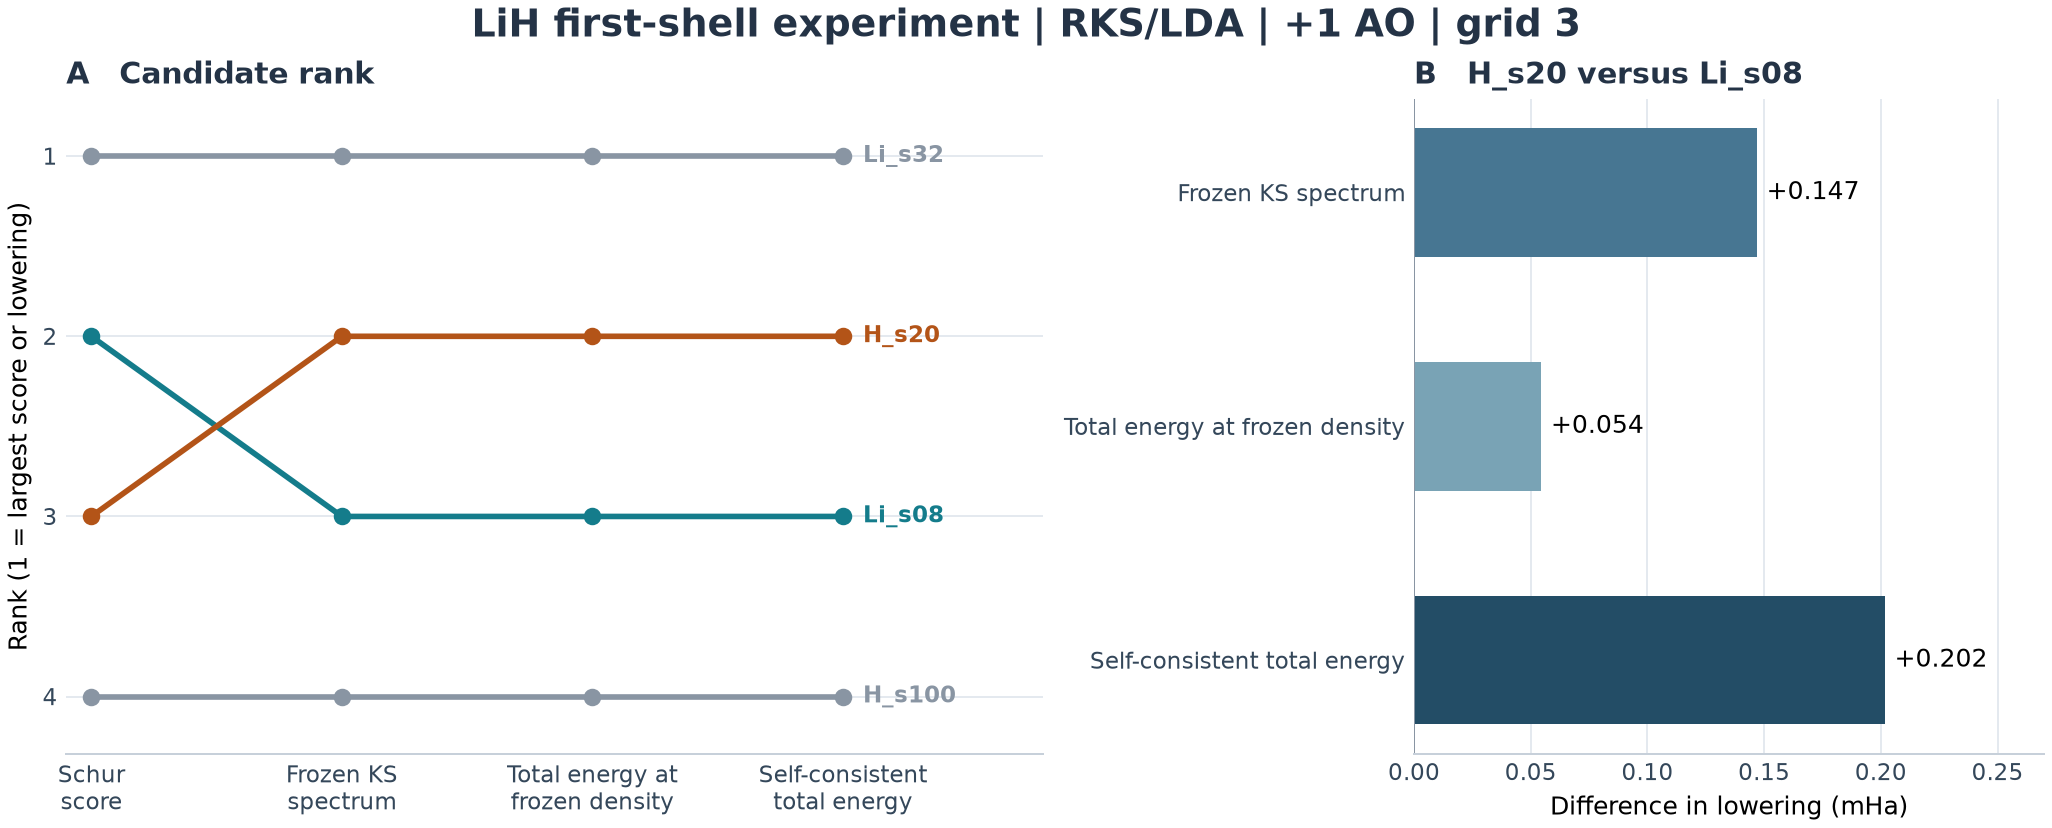
\includegraphics[width=\linewidth]{evidence/stage4/ranking.png}
\par\smallskip
{\small 图 1\quad 网格 3 的四个候选，以及 \code{H_s20} 相对 \code{Li_s08} 的能降差。\\
图据 \code{evidence/stage4/results/15/stage4_probe.json} 绘制。}
\end{center}

网格 3 上，\code{H_s20} 相对 \code{Li_s08} 的冻结谱、冻结密度总能量及重新自洽总能量降幅优势分别为 \FrozenMargin{}、\DensityMargin{} 和 \ScfMargin{} mHa。名次交换已发生于固定旧密度后的线性本征问题。原字典上的三种策略同选 \code{Li_s32}，删去它后在网格 3 与 4 同选 \code{Li_s08}。穷举显示后者的重新自洽能量约比 \code{H_s20} 高 \ScfMargin{} mHa。进一步仅改变 \(\gamma\in\{0.25,0.5,1.0\}\) 时，六次观测的 Li 减 H 原子平方指标介于 \(\SmallestAtomGap\) 与 \(\LargestAtomGap\) 之间，选择仍然一致。

初始、删壳对照及权重扫描命令分别耗时 \FirstSeconds{}、\AblationSeconds{}、\SweepSeconds{} 秒，包含进程启动和 I/O。相关拟合均记录收敛、AO 数、格点指纹和条件数。权重扫描复用同一组单壳自洽结果，因此直接测到的是局部化权重对选择的影响。

\subsection{结论与可验证问题}
在给定 LiH 几何、有限高斯候选及同 AO 预算内，Schur 分数提供了可计算的基组方向信息。已出现分数排名与重新自洽能量排名不一致的样本。所测设置下，额外的原子筛选暂未改善候选选择。下一步可检验更宽权重区间、更多体系或不同候选字典，或比较带谱曲率信息的排序指标。要把有限维条件上界推进到一般自洽估计，还需验证切空间逆算子的稳定常数、非线性余项和更大空间的对偶残差尾项。近似参考敏感性与连续基组极限之间的差距也尚待量化。

\clearpage
\section{复现与仓库材料}
\subsection{关键命令}
以下从项目根目录执行，依赖安装与 Windows 下载 Linux wheel 的实际恢复步骤见 \code{docs/numerics.md} 和 \code{docs/agent.md}。采用新的输出目录，正式结果的归档位于 \code{evidence/}。
\begingroup\small
\begin{verbatim}
# PowerShell  智能体环境、启动与报告构建
py -3.13 -m venv .venv
.\.venv\Scripts\python.exe -m pip install -r requirements-agent.txt
$cfg = 'config/agent.stage4.json'
.\.venv\Scripts\python.exe -m ksagent --config $cfg `
    --run-dir runs/report-check --transport https
pwsh -File scripts/build_report.ps1

# Linux 或 WSL  数值基线与阶段 4 归档版本
bash scripts/run_stage3.sh runs/check-stage3
bash scripts/reproduce_stage4.sh 13 runs/check-stage4/first.json
bash scripts/reproduce_stage4.sh 20 runs/check-stage4/ablation.json
bash scripts/reproduce_stage4.sh 31 runs/check-stage4/sweep.json
\end{verbatim}
\endgroup
\noindent 科学脚本默认使用 \code{.venv-science}。依赖见 \code{requirements-numerics.txt}。报告构建使用 XeLaTeX 和 Fandol 中文字体。

\subsection{证据定位}
\noindent\begin{tabularx}{\linewidth}{@{}lY@{}}
\toprule
目录或文件 & 用途\\
\midrule
\code{ksagent/}, \code{config/} & CLI、模型适配、工具、研究范围与实验配置。\\
\code{experiments/}, \code{scripts/} & 数值模型、增广策略、绘图、复现和报告构建。\\
\code{evidence/stage3/} & 基线 JSON/JSONL、同预算 CSV、敏感性和两个负对照。\\
\code{evidence/stage4/} & 真实事件、检查点、审计、代码版本、实际输出与图。\\
\code{report/}, \code{output/pdf/} & XeLaTeX 源文件、生成数字的程序与成品。\\
\bottomrule
\end{tabularx}

\subsection{复现验收}
核对阶段 3 的累计 AO 数、能量偏差、格点指纹和两套参考。实验失败对照应保留非零状态和诊断。阶段 4 的科学重算可使用行动 13、20 和 31 的三个归档版本。比较重新生成的科学字段，时间字段单独记录。需要核对智能体因果链时，先在审计表中找到行动号，再对照原始事件、代码版本和哈希匹配的产物。报告数字由 \code{report/generate_data.py} 从结果和日志读取并核对，不依赖新的模型调用。

\clearpage
\section{相关工作与阅读边界}
最接近本题的两条线索是线性全空间 LCAO 局部可靠性 \cite{dupuy} 和分子高斯轨道基的基组极限研究 \cite{jensen}。前者需要局部稳定性、谱分离和尾项控制，后者提供逐级比较参考的思路。非线性有限元与 DG 估计分别提供切空间条件及局部插值和界面条件的类比 \cite{chen,kaye}。这些条件在本项目的全局重叠高斯函数上需要单独建立。

冻结算符的谱分离与非线性响应在文献中对应不同的论证 \cite{herbst,cances}。智能体实际读取了第二篇的公开摘录，据其中的逆 Jacobian 讨论决定在实验里分项测量。出版社拦截的正文仅记录为访问失败。检索日期为 2026 年 11 月 21 日，覆盖范围和阅读位置见 \code{docs/literature.md}，其中另记了软件实现资料与 Crossref 题录查询。

\begingroup
\small
\renewcommand{\refname}{参考文献与查阅位置}
\begin{thebibliography}{9}
\bibitem{dupuy} M.-S. Dupuy, G. Dusson, I.-M. Lygatsika. A posteriori error estimates for Schrödinger operators discretized with linear combinations of atomic orbitals. \href{https://doi.org/10.1137/24M1700697}{期刊}，\href{https://arxiv.org/html/2410.04943}{公开稿}。查阅摘要、§3.1 与 §4.1.4--4.1.5。
\bibitem{chen} H. Chen, X. Dai, X. Gong, L. He, A. Zhou. \href{https://doi.org/10.1137/130916096}{Adaptive finite element approximations for Kohn--Sham models}。查阅残差、A3 和收敛段。
\bibitem{kaye} J. Kaye, L. Lin, C. Yang. \href{https://math.berkeley.edu/~linlin/publications/APostKSDFT.pdf}{A posteriori error estimator for adaptive local basis functions to solve Kohn--Sham density functional theory}。查阅式 (3.16)--(3.17) 及定理 3.5。
\bibitem{herbst} M. F. Herbst, A. Levitt, E. Cancès. \href{https://arxiv.org/abs/2004.13549}{A posteriori error estimation for the non-self-consistent Kohn--Sham equations}。查阅谱间隙估计和数值讨论。
\bibitem{cances} E. Cancès, G. Dusson, G. Kemlin, A. Levitt. \href{https://arxiv.org/html/2111.01470}{Practical error bounds for properties in plane-wave electronic structure calculations}。定向查阅逆 Jacobian 与线性化框架。智能体实际读取 HTML 偏移 0--14000。
\bibitem{jensen} F. Jensen. \href{https://doi.org/10.1063/1.1465405}{Polarization consistent basis sets II. Estimating the Kohn--Sham basis set limit}。查阅分级构造与外推。
\bibitem{pyscf} PySCF. \href{https://pyscf.org/contributor/scf_developer.html}{SCF 开发者文档}与 \href{https://pyscf.org/_modules/pyscf/dft/rks.html}{RKS 实现}。查阅密度输入、有效势与网格。
\end{thebibliography}
\endgroup
\end{document}
